\section{香港真的實行三權分立嗎?}

香港政治其中一個奇謬之處,是同樣對香港極有影響力的官員,可以對香港的政治體制有極為不同理解,使得政治辯論往往連最基本的共識都不存在。前中聯辦主任張曉明曾在二零一五年聲稱香港實行的不是三權分立制度,行政長官有超然於行政、立法和司法的法律地位,引起一時輿論熱議。有傳媒則翻出香港兩任終審法院首席法官李國能和馬道立過去的言論,他們均曾清楚表明三權分立是香港政治制度的重要基礎。有傳媒就張曉的言論訪問馬道立法官,他便引用了《基本法》中司法獨立和人人平等的條文作回應。

解釋他們的理解為何會有出入之前,得先釐清三權分立的意思。政治學上的權力分立是指把公權力分散在不同機關當中,以產生互相制衡作用。以行政權、立法權和司法權為劃分的三權分立,就是一種常見的權力分立制度。其中,行政權和立法權分割的程度在不同政治體制有別。例如在美國的總統制當中,行政權和立法權就全面分割,選民分別選出總統和國會,由總統領導行政機關,受國會監督。在一個三權分立的制度中,行政權執行政策,管理政府的日常運作;立法會監督行政權,通過立法和審批財政等方式規範行政權;司法權則擔當仲裁角色,如裁決行政當局有否違法和議會通過的法案有否違憲。這樣的設計來自法國啟蒙思想家孟德斯鳩,他認為通過權力相互制約同避免任何一方獨斷獨行,為人民帶來災難。

香港的政治制度設計上類近美國的總統制,同樣分行政權、立法權和司法權,行政長官和立法會分開選出。行政長官領導行政機關,也就是特區政府。《基本法》例明行政長官和行政機關受立法會和司法機關的監督,而立法會本身也受司法機關的監督。至於司法機構當中終審法院的法官和高等法院首席法官的任命或免職,則又需要行政長官和立法會的同意。

\begin{figure}[htbp]
    \centering
    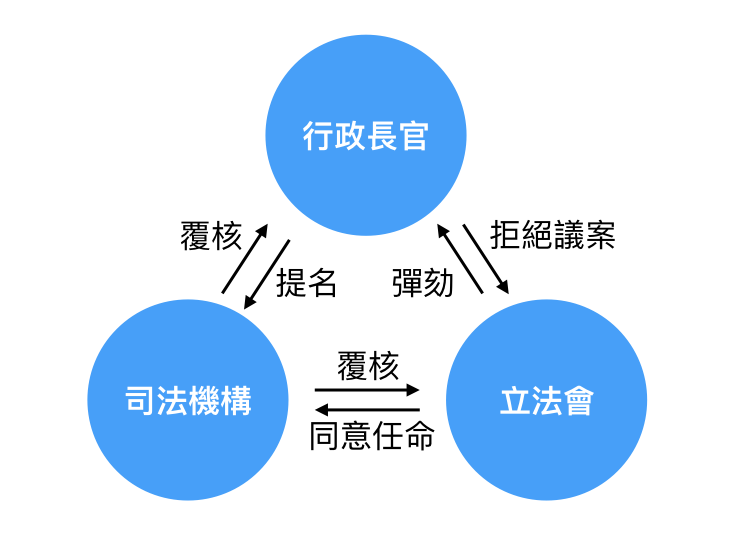
\includegraphics[width=0.7\textwidth]{c15/h-klesson1-021.png}
    \caption{簡化版的香港「三權分立」} 
\end{figure}

雖然在《基本法》的條文中沒有出現過「三權分立」這四個字,但處處可見三權分立的操作。《基本法》第四十八條、第四十九條、第五十條、第五十二條和第七十六條所述的行政長官和立法會職權,可看到權力相互制約。政府提出的法案要交由立法會審議通過,而立法會通過的法案又要得到行政長官的簽署才能成為法律。如果行政長官拒絕簽署立法會通過的法案,可以在三個月內將法案發回重議;但如果法案再獲立法會不少於全體議員三分之二多數通過,則行政長官只可以選擇簽署或解散立法會。不過,如果重選後該法案仍然獲立法會不少於全體議員三分之二多數通過,則行政長官必須辭職。上述的情況在特區成立以來沒有出現過,實際上發生的可能性也甚低,但這些條文的存在足以說明《基本法》認同權力應該相互制約。

在政治實踐當中,自特區成立以來也出現過不少重大議案未獲立法會通過的案例,如2005年和2015年的政改方案就被否決。市民通過司法覆核嘗試推翻政府或立法會決定的案件更是無日無之,也曾有不少覆核成功的案例,如前文提及港珠澳大橋工程環境許可證的覆核。至於「行政長官地位超然」的說法,容易讓人以為是指行政長官完全不受制約,不符《基本法》第二十五條列明「香港居民在法律面前一律平等」的規定,事實上前任行政長官曾蔭權於卸任後,亦因任期內違反「公職人員行為失當」罪名而被判監。這些事例都讓香港市民有理由相信,香港有一定程度上的三權分立。

話雖如此,香港的三權分立有不少明顯缺陷。

首先,相對於其他三權分立的政治制度,《基本法》給予行政權的權力比立法權明顯要多,所以香港政制常有「行政主導」之說。例如在美國,財政預算案的草議和審批權都在國會,總統極其量只可以拒絕簽署發還重議;在香港則剛好相反,財政預算案的草議權在政府一方,立法會只能選擇通過或否決。因此,香港的立法會議員利用財政預算來改變政府政策的能力,就遠遠低於美國的國會議員。此外,《基本法》第七十四條規定立法會提出法律草案時,不得「涉及公共開支或政治體制或政府運作」,而「凡涉及政府政策者,在提出前必須得到行政長官的書面同意」。僅是這一條,就決定了政策設定的權力完全傾向行政權一方。立法會議員想提出一些政府沒打算提出的政策,就連門也沒有。

第二,香港不是一個獨立政體,《基本法》為中央政府保留不少介入香港的政治的權力:

\begin{itemize}
    \item 按《基本法》第十七條,全國人大常委會如果認為立法會通過的法律「不符合本法關於中央管理的事務及中央和香港特別行政區的關係的條款」,可將有關法律發回,該法律在香港即告失效。
    \item 按《基本法》第四十五條,行政長官在香港通過選舉或協商產生,然後由中央人民政府任命,而普遍的理解是中央政府有權不任命。
    \item 按《基本法》第七十九條第九項,雖然立法會有權彈劾行政長官,但就算議案得到立法會以全體議員三分之二多數通過,仍然要報請中央人民政府決定,即中央政府有權推翻立法會通過的彈劾。
    \item 按《基本法》第一百五十八條的規定,《基本法》的解釋權屬於全國人民代表大會常務委員會。自特區成立以來,對此條文的理解已變成是人大常委可在任何時候解釋《基本法》,而香港的司法機關都會執行這解釋。
\end{itemize}

由此可見,香港政治不只是三權之間的互相制約,中央政府在必要是可以大幅甚至完全削去一些行政權、立法權或司法權的權力。其中行政長官的任命和彈劾要由中央政府決定,正正就是所謂「行政長官超然」說法的依據,意謂行政長官的地位並不完全受香港的立法會和司法機關的制約,和正常三權分立的政體有別。

最後,從實際操作上看,權力制約背後假設了權力來源分散,而這點在香港有明顯缺陷。自特區成立以來,由於政治制度和實際操作所限,不管香港主流民意為何,結果無論是行政長官或是立法會的多數議員的政治立場均親北京。由於行政和立法雙方都是同一陣營而又沒有下台的憂慮,有效的互相制約就無從發生。而對於司法機關來說,就算他們嘗試保持獨立,也要按現存的政治和法律制度行事。如果制度本身有缺陷,司法機關可做的事情十分有限。在上述的重重困難下,香港的三權分立就很容易變得有形無實了。



伸延閱讀:

Gittings D (2016) System of Government, Introduction to the Hong Kong Basic Law (2nd Edition). Hong Kong: Hong Kong University Press.

Lo PY (2014) The Background of Concepts, The Judicial Construction of Hong Kong’s Basic Law: Courts, Politics and Society after 1997. Hong Kong: Hong Kong University Press.